\pagebreak
\section{Anhang}
\label{sec:Anhang}


\begin{figure}
    \centering
    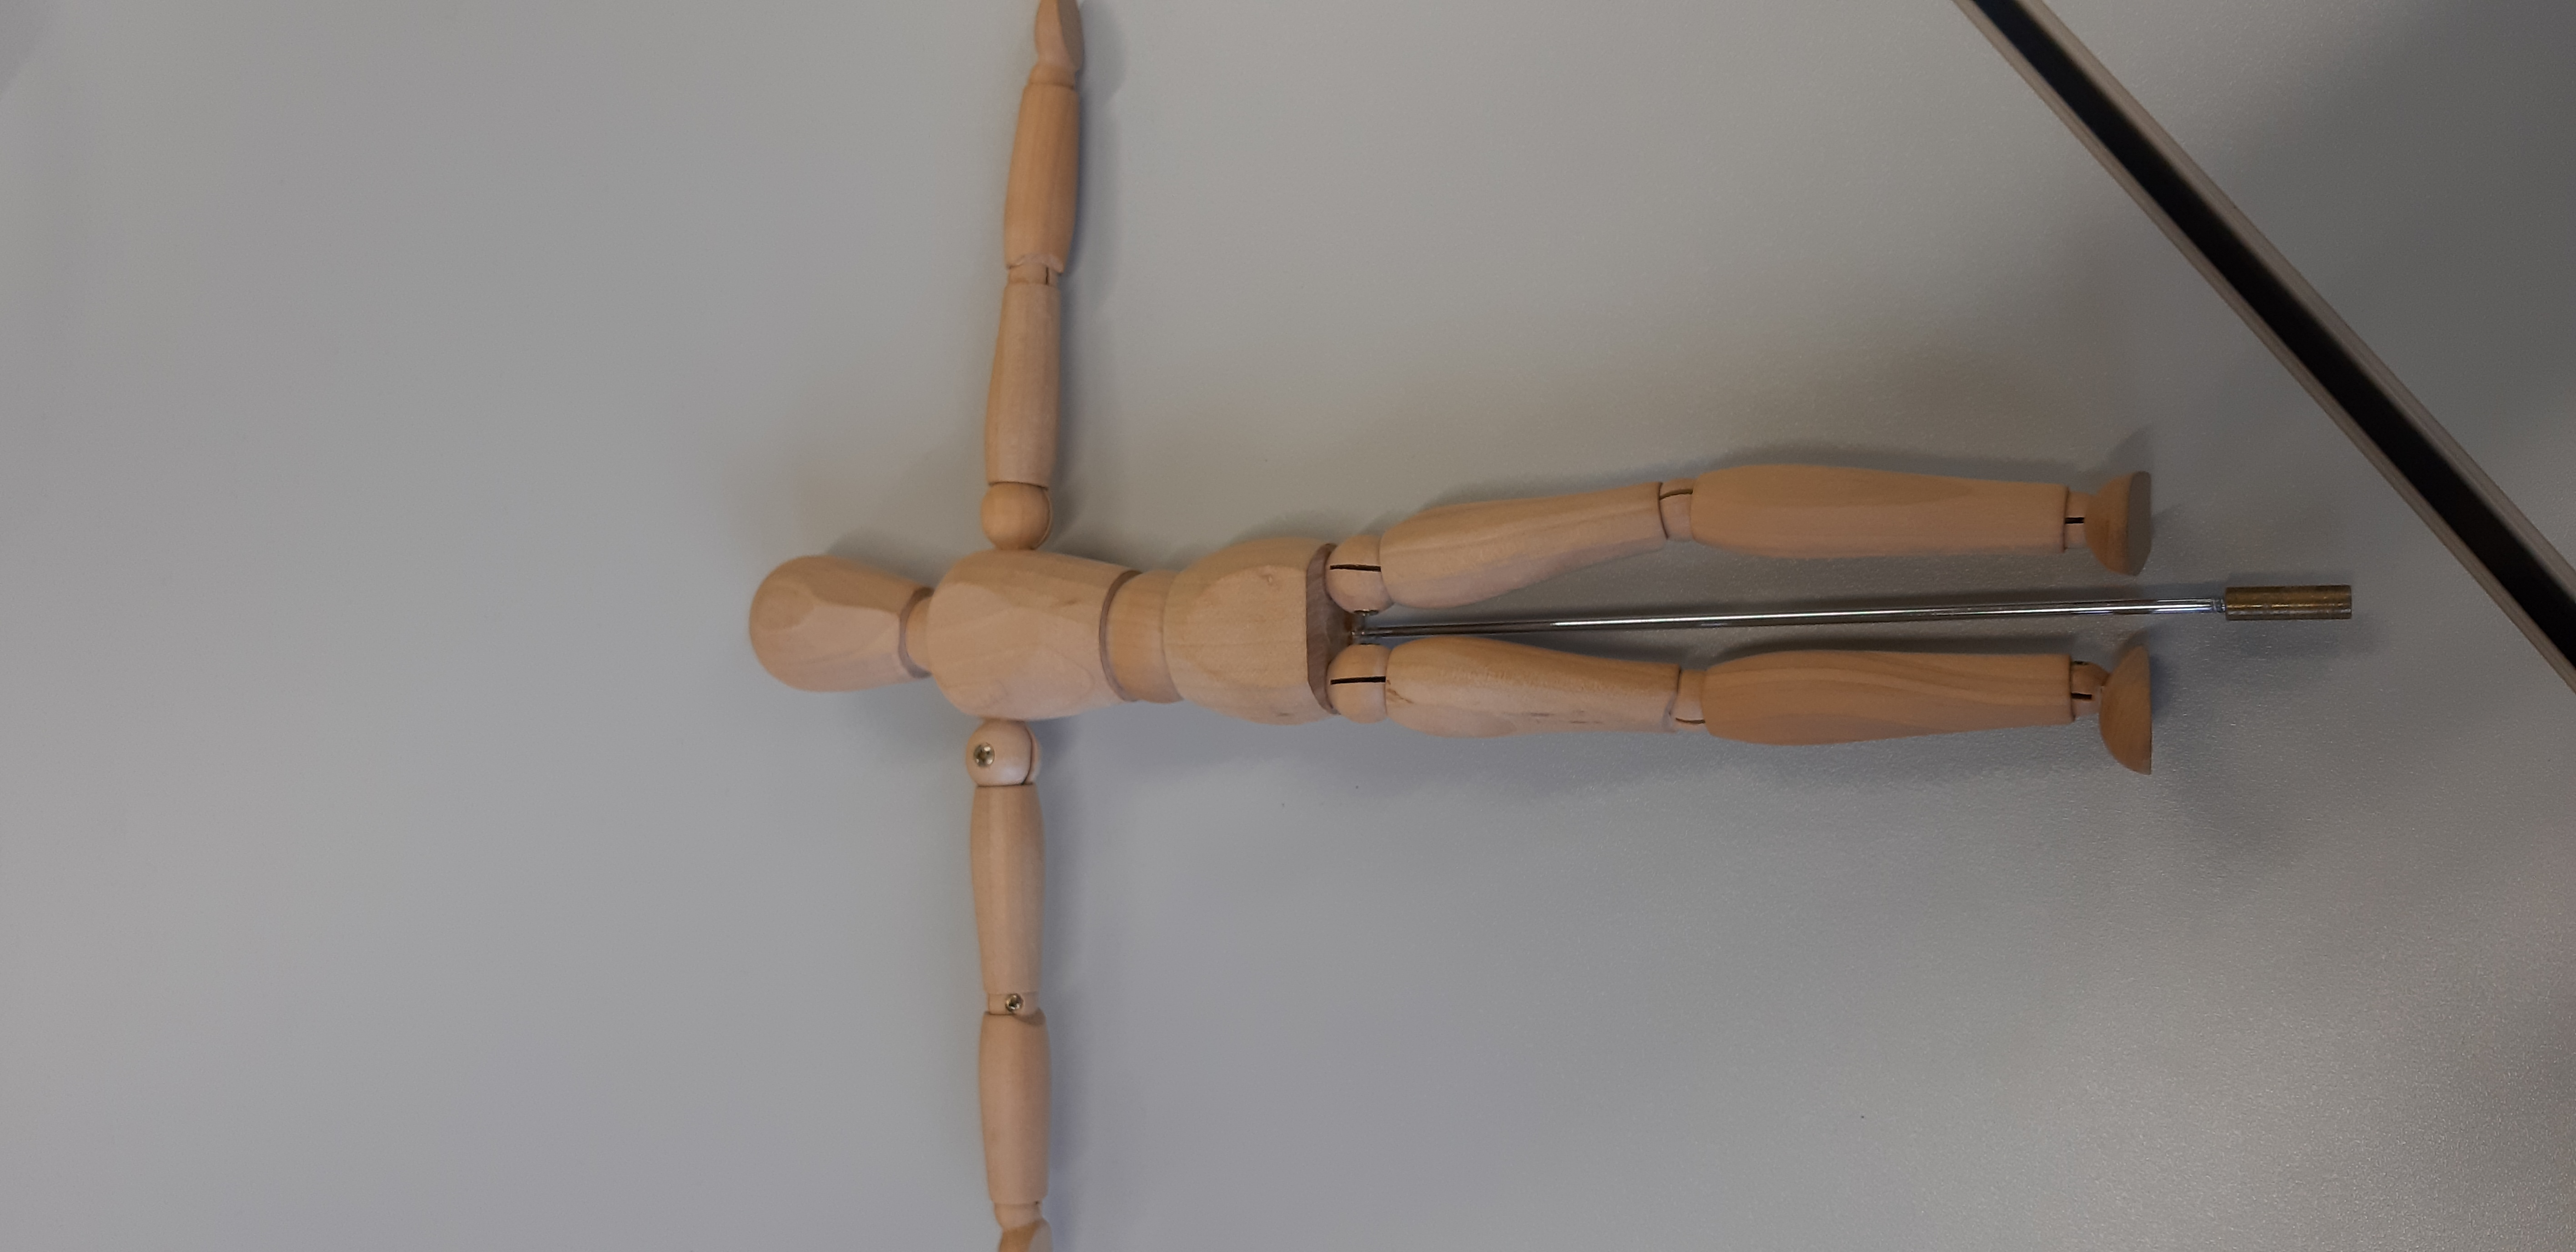
\includegraphics[width=0.75\textwidth, angle=-90]{Bilder/Stellung1.jpg}
    \caption{Erste Stellung der Puppe}
    \label{fig:stellung1}
  \end{figure}
  
\begin{figure}
  \centering
  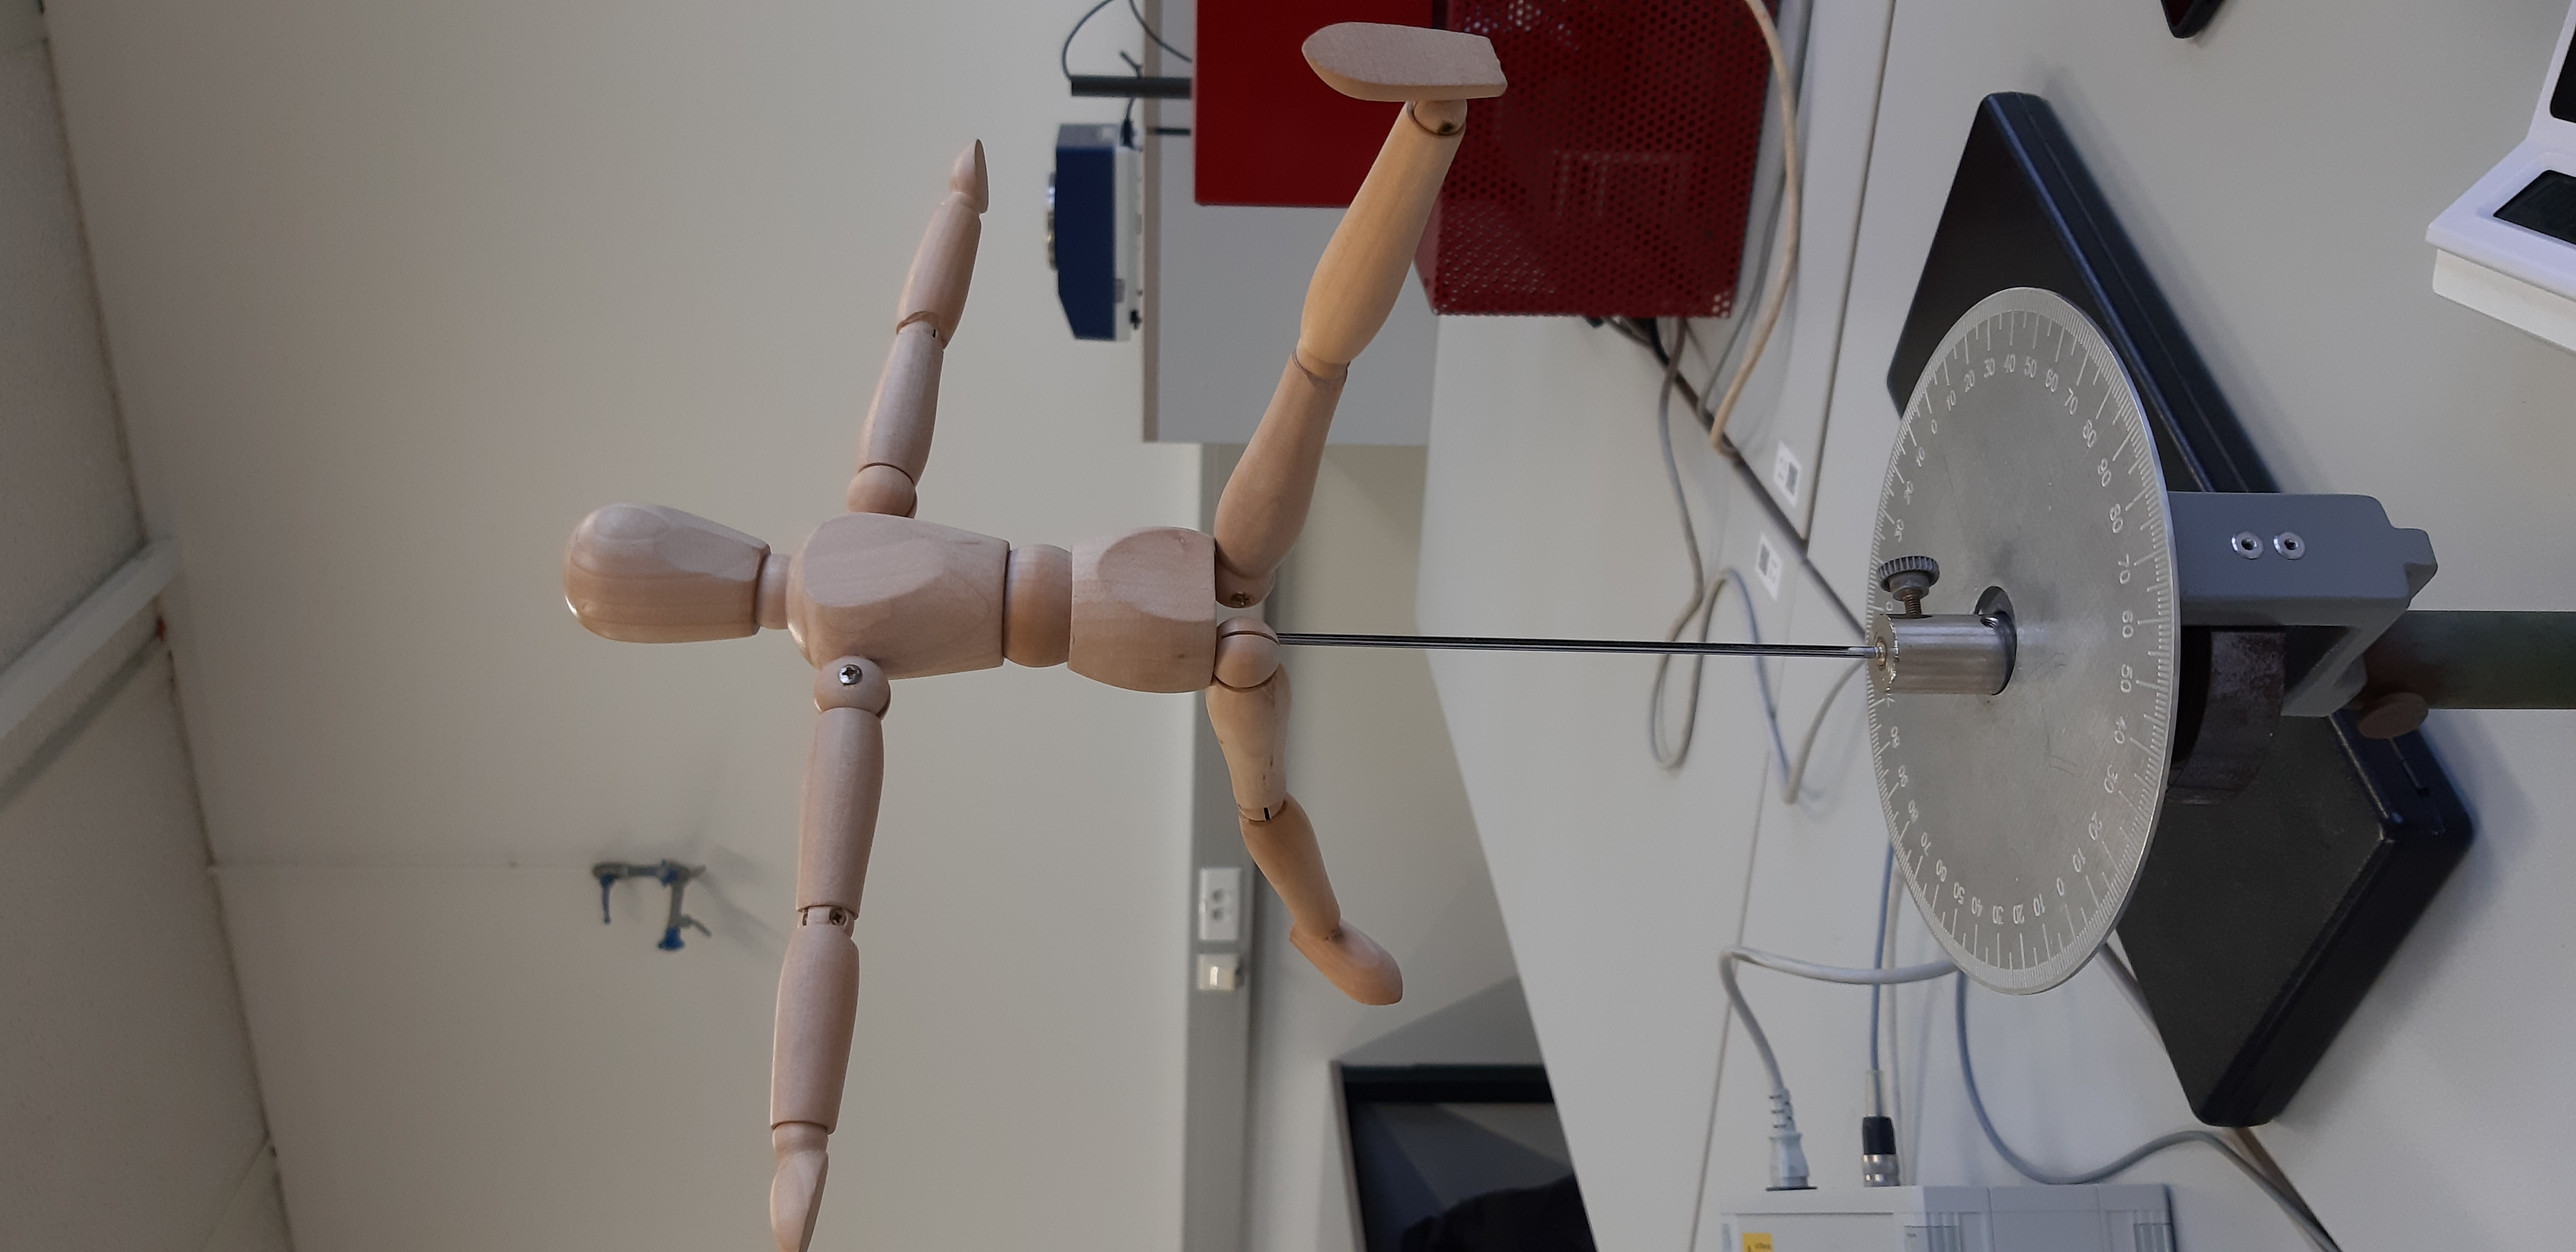
\includegraphics[width=0.75\textwidth, angle=-90]{Bilder/Stellung2.jpg}
  \caption{Zweite Stellung der Puppe}
  \label{fig:stellung2}
\end{figure}

\begin{figure}
  \centering
  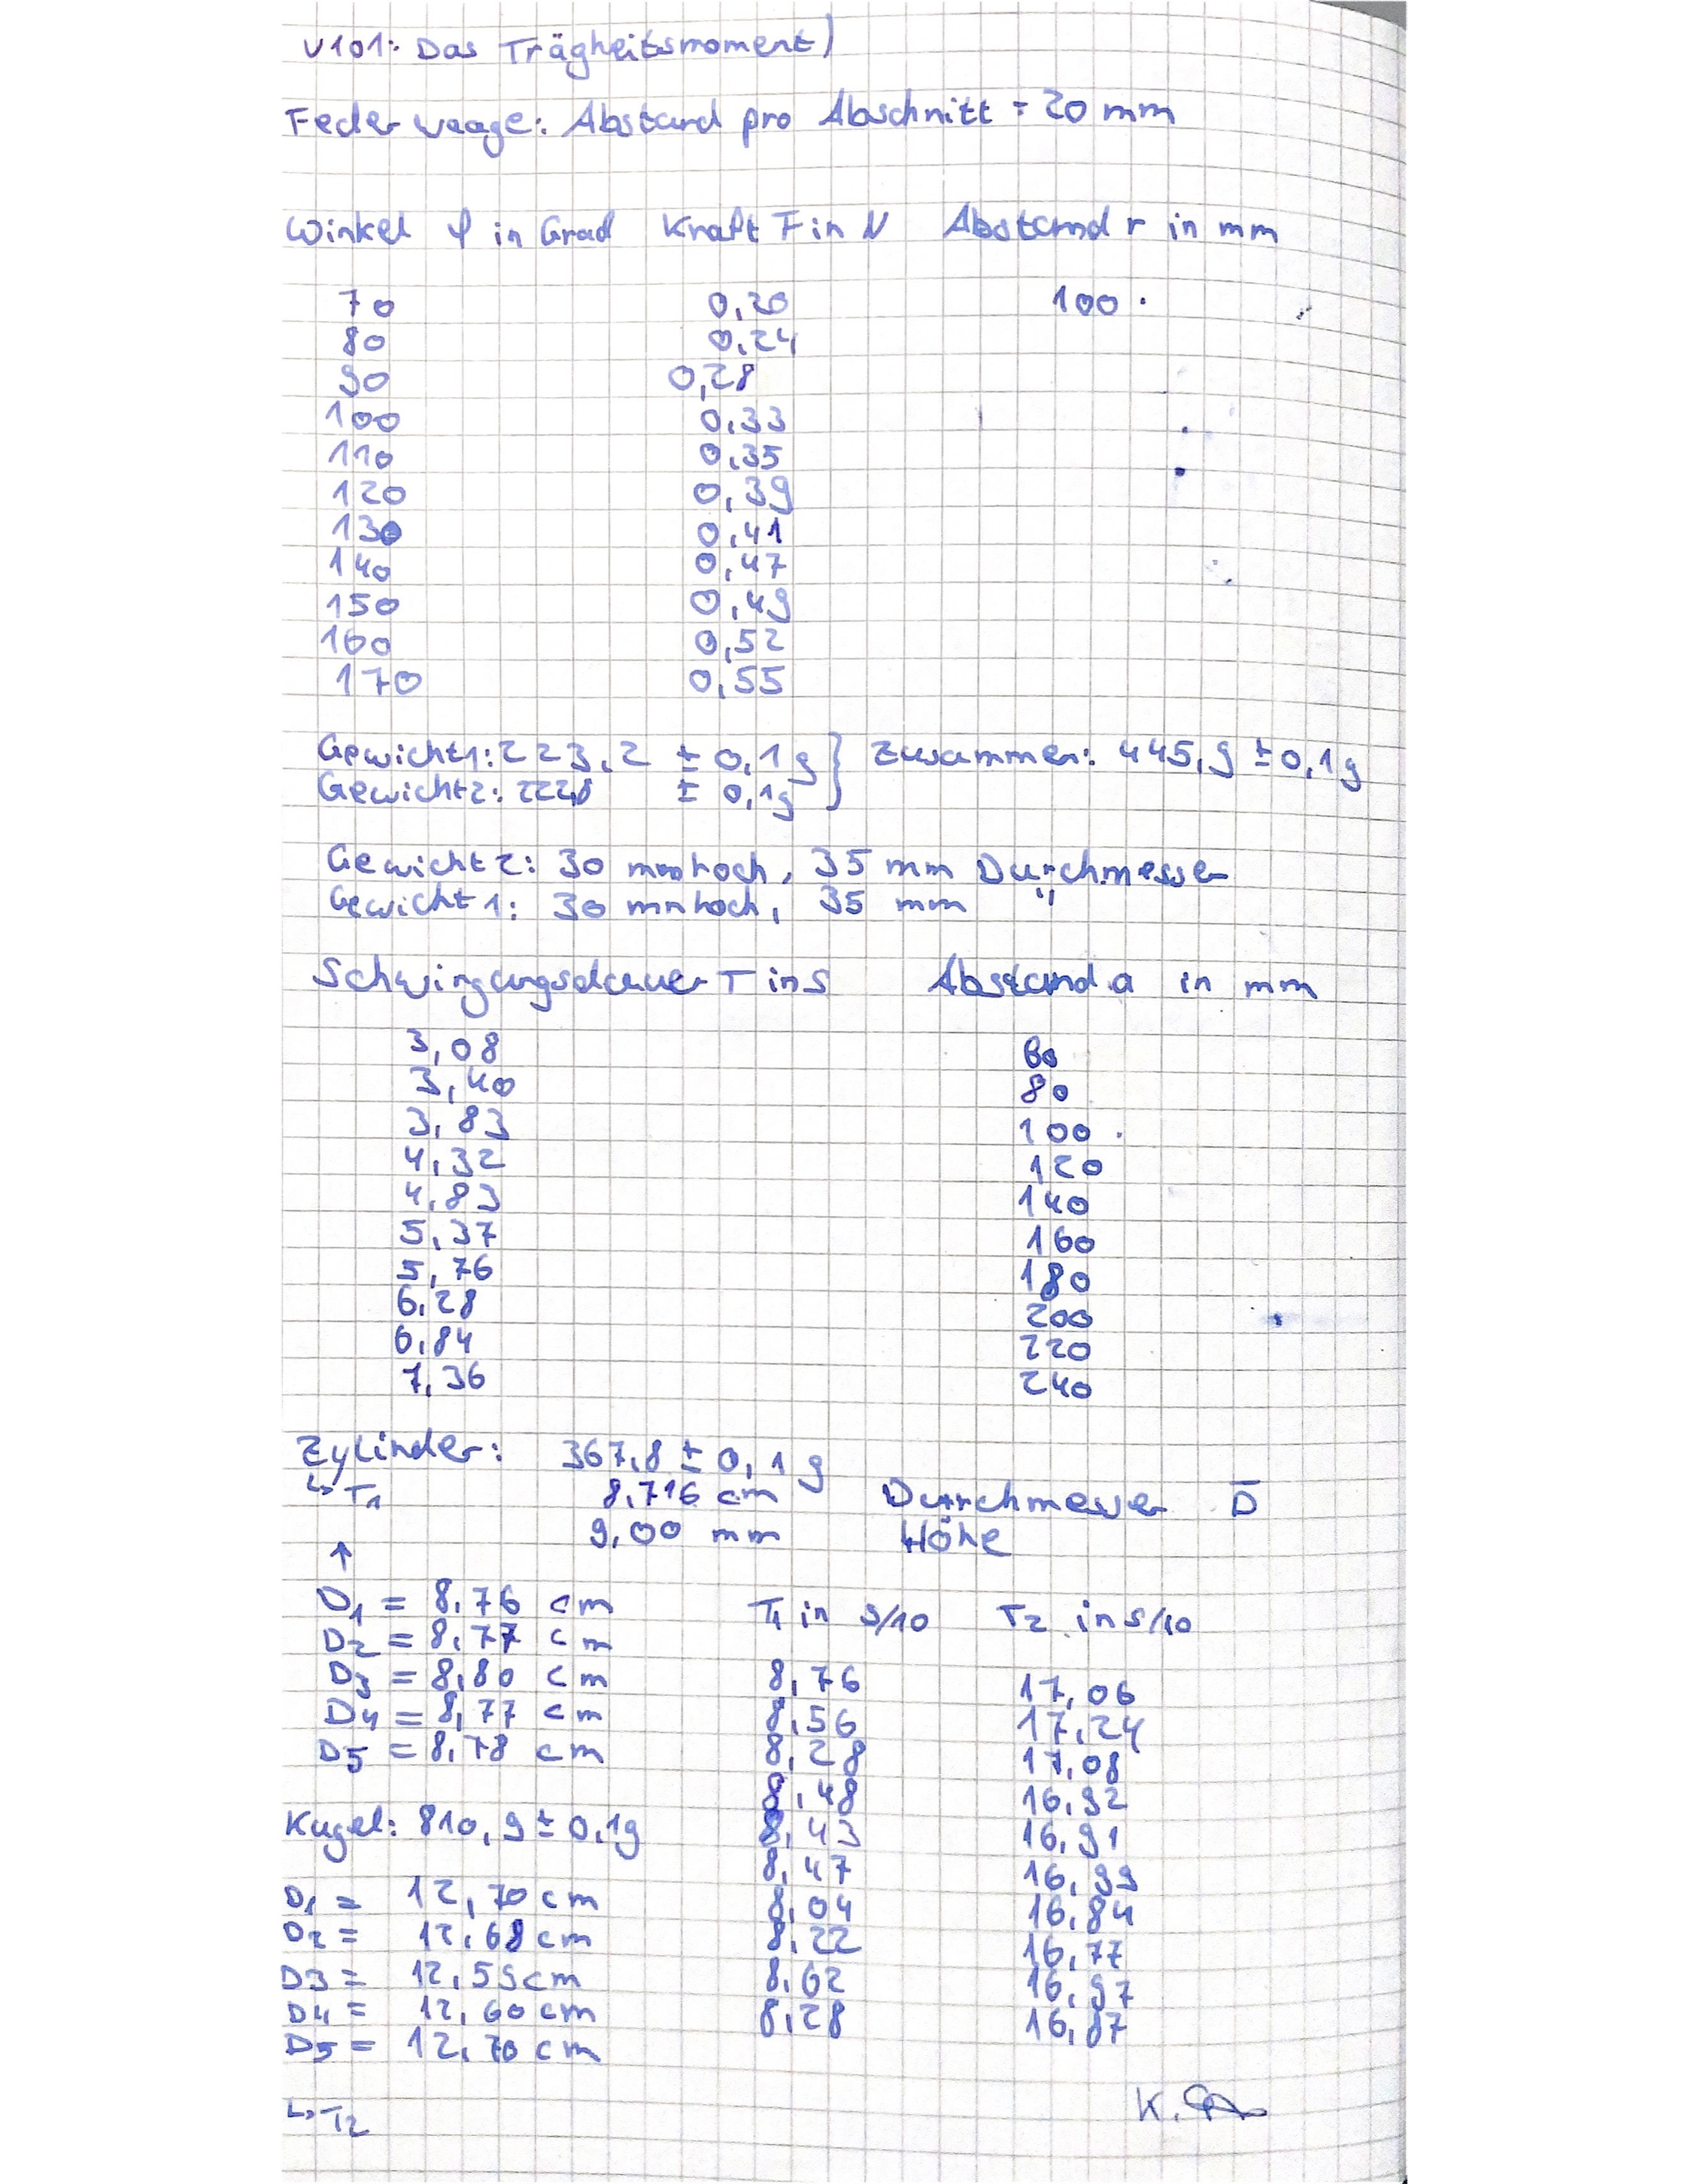
\includegraphics[width=0.75\textwidth]{Bilder/daten1.jpg}
  \caption{Originale Messdaten}
  \label{fig:daten1}
\end{figure}

\begin{figure}
  \centering
  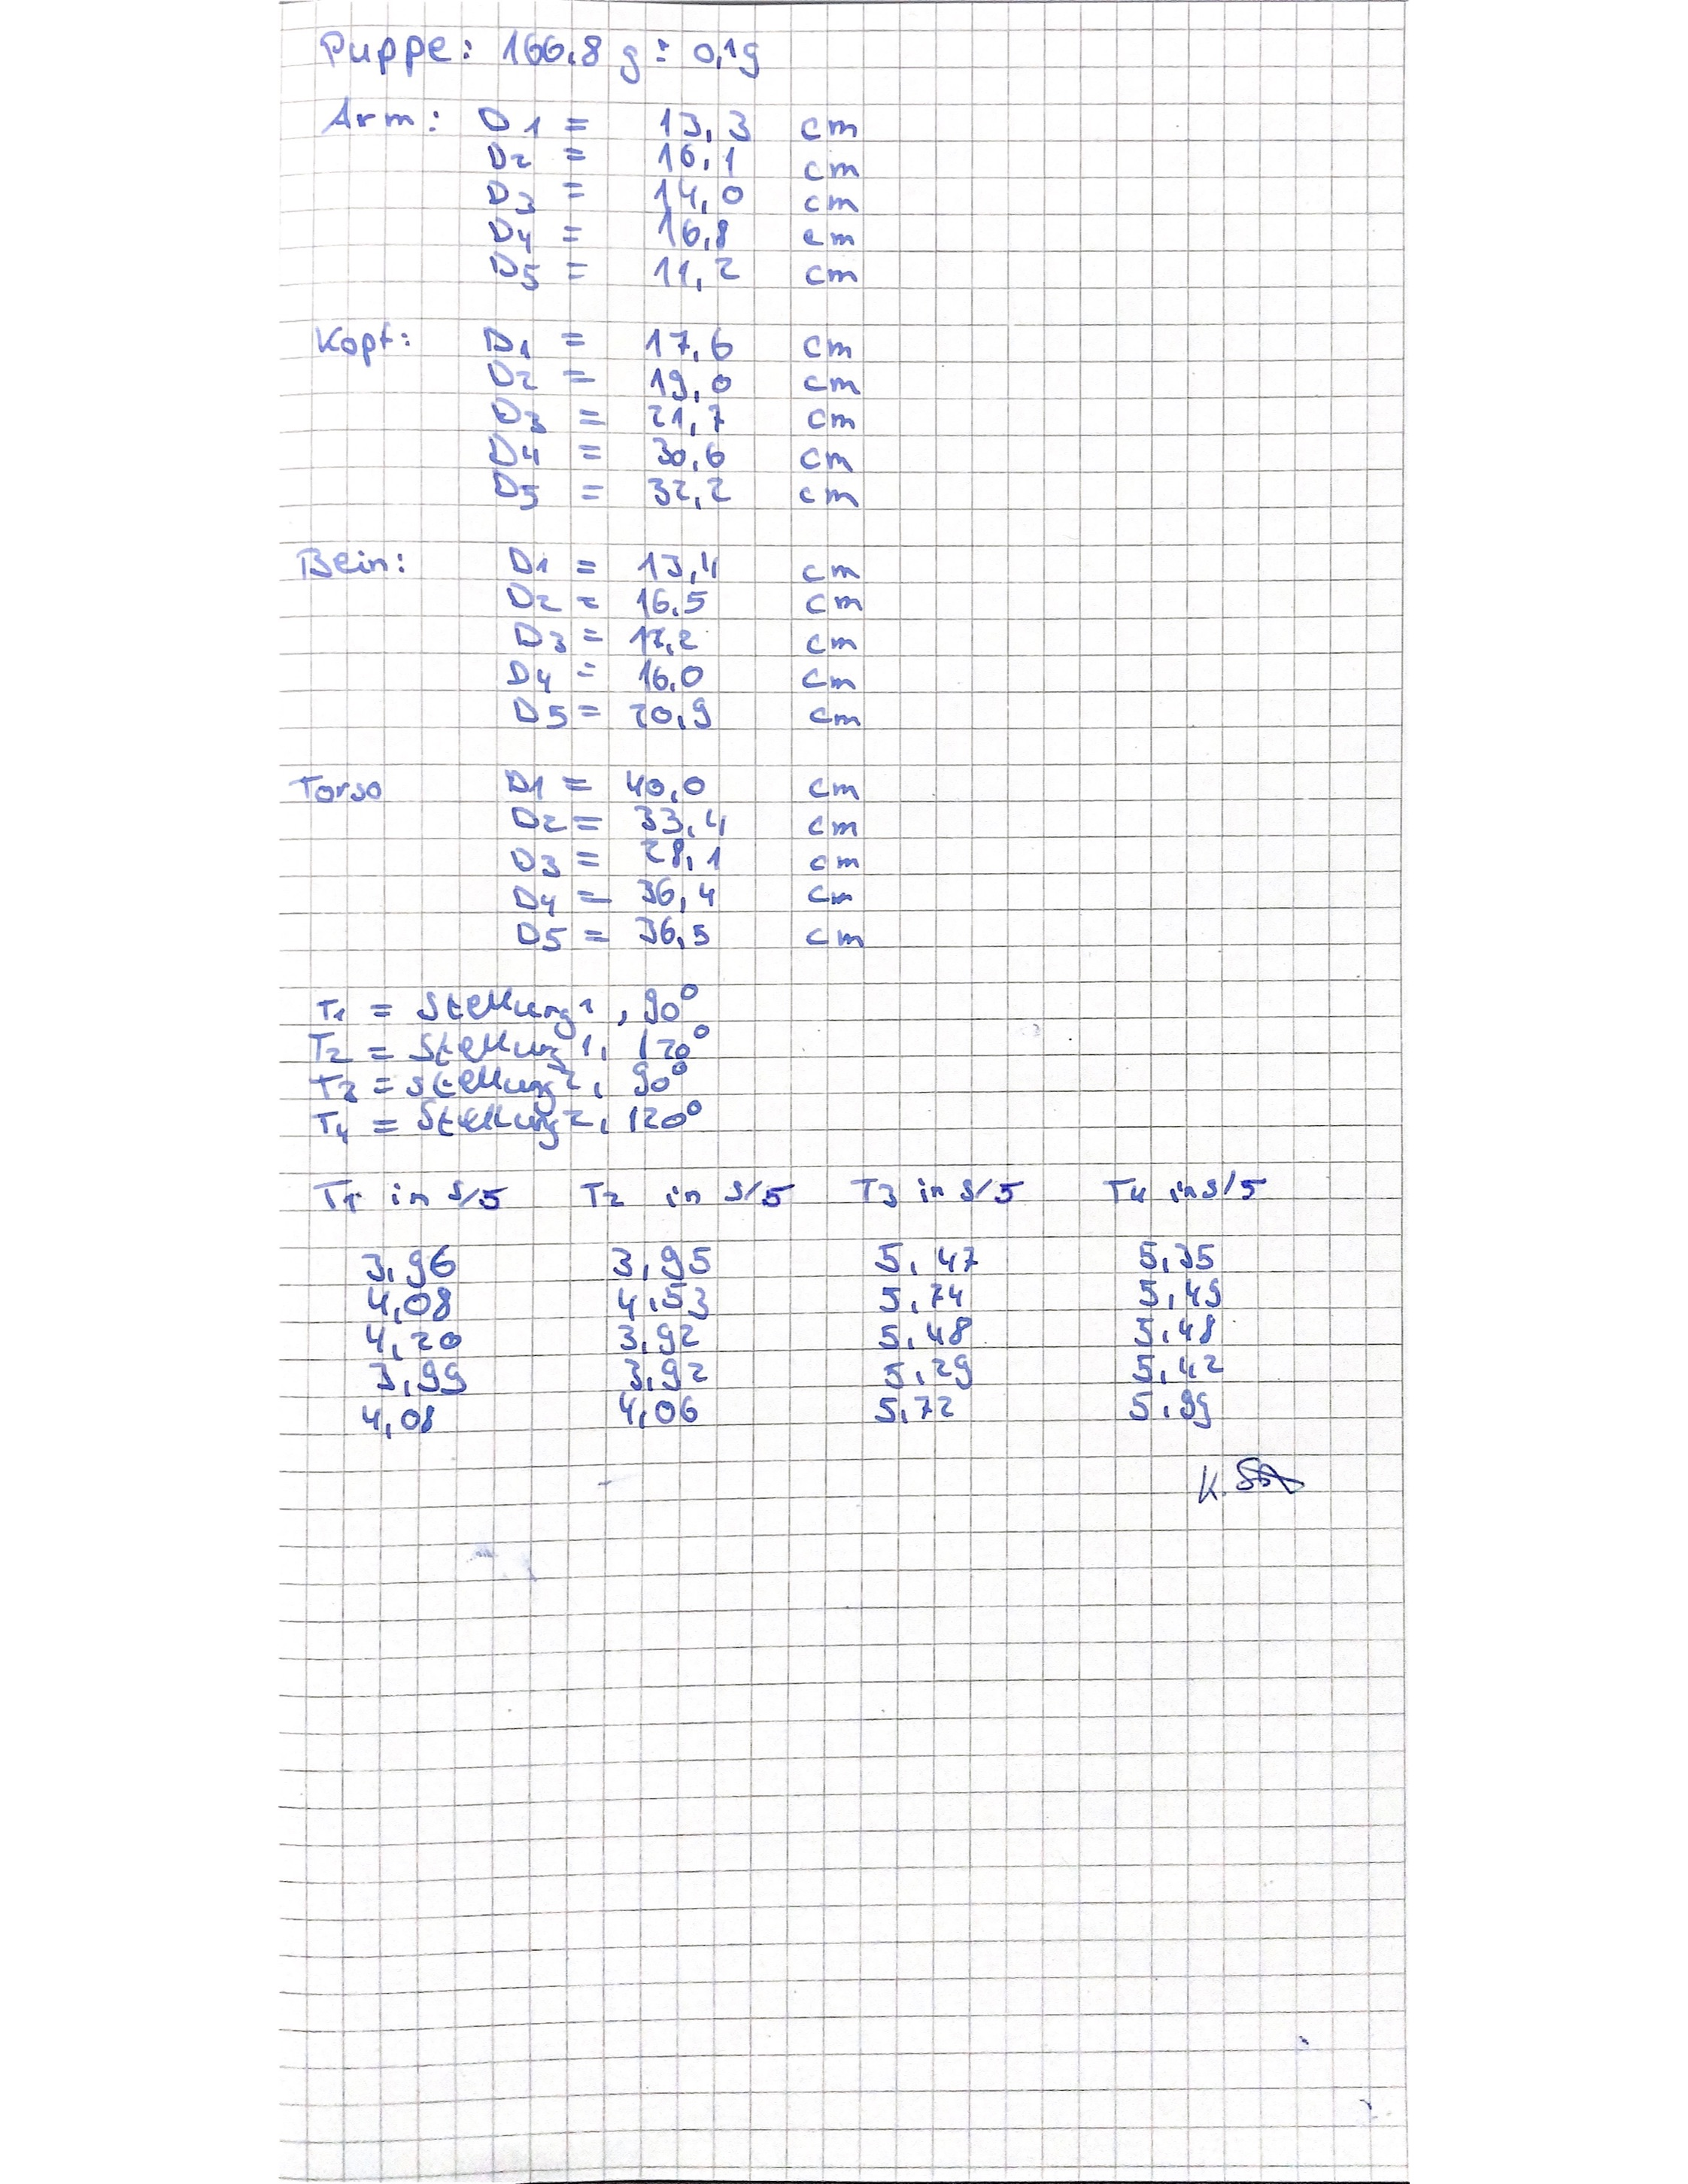
\includegraphics[width=0.75\textwidth]{Bilder/daten2.jpg}
  \caption{Originale Messdaten}
  \label{fig:daten2}
\end{figure}